\documentclass[crop,tikz]{standalone}% 'crop' is the default for v1.0, before it was 'preview'
%\usetikzlibrary{...}% tikz package already loaded by 'tikz' option
\usetikzlibrary{shapes,snakes}
\usepackage{amsmath}
\begin{document}
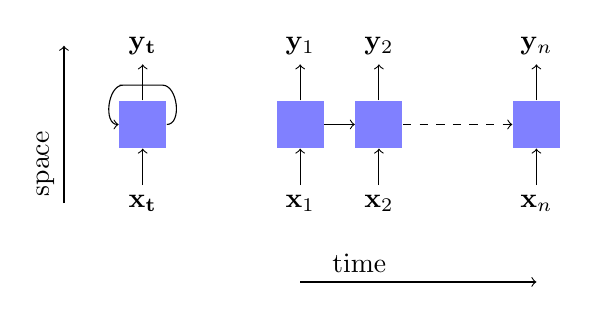
\begin{tikzpicture}

\def\layersep{1.0cm}

\tikzstyle{rcNeuron}=[rectangle,fill=black!25,minimum size=17pt,inner sep=0pt]
\tikzstyle{LSTM}=[rcNeuron, fill=blue!50];
\tikzstyle{neuron}=[rectangle,fill=black!25,minimum size=17pt,inner sep=0pt]
\tikzstyle{linearNeuron}=[neuron, fill=green!50];
%Layer Marks
\draw[->] (3*\layersep,0) -- (6*\layersep,0) node[near start, above] {time};
\draw[->] (0,\layersep) -- (0,3*\layersep) node[near start, above,rotate=90] {space};


\node (x) at (1,1*\layersep) {$\mathbf{x_t}$};
\node[LSTM] (lstm1) at (1,2*\layersep) {};
\node (y) at (1,3*\layersep) {$\mathbf{y_t}$};

\draw[->] (x) -- (lstm1);
\draw[->] (lstm1) -- (y);

\draw[->] (lstm1) to[out=0,in=0] (1.25,2.5*\layersep) to[out=180,in=180] (0.75,2.5*\layersep) to[out=180,in=180]  (lstm1);


\node (xt) at (3,1*\layersep) {$\mathbf{x}_{1}$};
\node[LSTM] (unrolledLstm1) at (3,2*\layersep) {};
\node (yt) at (3,3*\layersep) {$\mathbf{y}_{1}$};

\node (xt2) at (4,1*\layersep) {$\mathbf{x}_{2}$};
\node[LSTM] (unrolledLstm1t2) at (4,2*\layersep) {};
\node (yt2) at (4,3*\layersep) {$\mathbf{y}_{2}$};

\node (xtn) at (6,1*\layersep) {$\mathbf{x}_{n}$};
\node[LSTM] (unrolledLstm1tn) at (6,2*\layersep) {};
\node (ytn) at (6,3*\layersep) {$\mathbf{y}_{n}$};

\draw[->] (xt) -- (unrolledLstm1);
\draw[->] (unrolledLstm1) -- (yt);

\draw[->] (xt2) -- (unrolledLstm1t2);
\draw[->] (unrolledLstm1t2) -- (yt2);

\draw[->] (xtn) -- (unrolledLstm1tn);
\draw[->] (unrolledLstm1tn) -- (ytn);


%horizontal connections.
\draw[->] (unrolledLstm1) -- (unrolledLstm1t2);
\draw[->,dashed] (unrolledLstm1t2) -- (unrolledLstm1tn);



\end{tikzpicture}
\end{document}